% 本文件是示例论文的一部分
% 论文的主文件位于上级目录的 `main.tex`
\chapter{利用粮食生产预测模型进行分析与验证}
\label{chapter:4}
本章主要对\ref{chapter:3}中得到的特征选择结果和约简数据集进行数值实验分析,通过将原数据集与约简数据集中2004-2020年的数据投入预测模型进行训练,并预测2021年各省份的产量,再与真实值进行比较,以便通过预测模型结果分析特征选择结果的优劣。
\section{预测模型数值实验}
\begin{figure}[!htb]
  \centering
  \resizebox{\textwidth}{!}
  {
  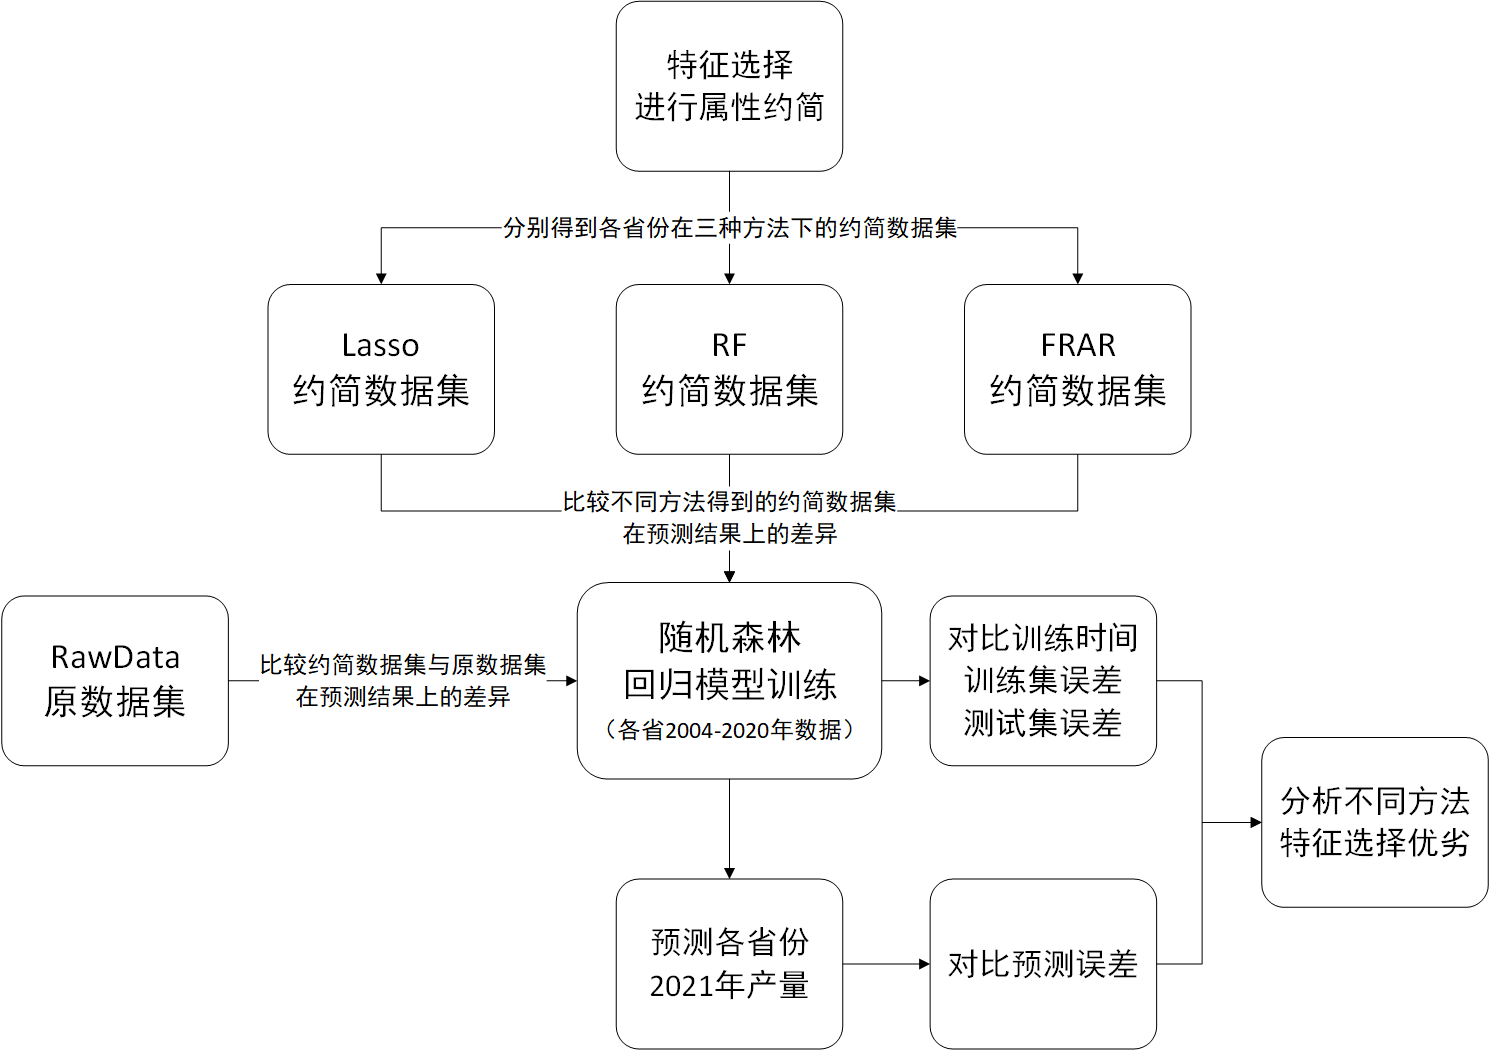
\includegraphics{PredictionVerification}
  }
  \caption{预测模型数值实验流程图}
  \label{fig:PredictionVerification}
\end{figure}

本章预测模型的数值实验主要目标是通过将不同特征选择方法得到的约简数据集放入预测模型,通过预测实验分析得到其模型的拟合效果与泛化能力,进而分析出约简数据集中特征的信息表现能力,以便对三种特征选择方法的特征选择结果进行评价与比较。

对于属性约简的评估方法,针对不同类型数据有着不同的评估方法。对于分类与回归问题,主要有决策树、随机森林、朴素贝叶斯、支持向量机、KNN等方法\cite{BestOverview}。本数值实验选择随机森林回归模型来作为预测模型对数据集进行实验分析。因随机森林变量重要性方法(RF)作为随机森林模型的一部分,其选择出的特征正是随机森林模型中对目标变量贡献最大的,因而将选出的特征放入模型进行试验将具有较优的拟合效果与表现。而随机森林模型自身在预测中本就有着较好的鲁棒性,因而可以将RF方法的实验结果作为一个较优的参考,进而可以据此来评价其余方法在预测模型中的表现,进而分析不同特征选择方法的特征选择效果。

本章数值实验的数据基于\ref{chapter:3}的三种特征选择方法的约简数据集与未约简原数据集,将每省的数据作为一个分析单元,横向对比同一省份不同数据集的预测效果,纵向分析不同省份相同预测模型指标的差异。以每省2004-2020年数据作为数据集,并将数据集按照8:2随机分为训练集与测试集,比较不同数据集在训练时间、训练误差、测试误差方面的差异,进而分析不同数据集在拟合效果方面的不同。然后将各省2021年的数据作为预测变量,预测各省2021年的作物产量,再与真实值比较得出预测误差,分析不同数据集在预测精度方面的优劣,进而得到不同数据集的泛化能力。最后综合比较约简数据集与未约简原数据集在预测模型表现上的差异,分析出在预测前将数据集进行属性约简对预测结果的影响,得到最终的实验分析结果。具体流程见\ref{fig:PredictionVerification}。

% 其中,预测数值实验具体算法流程见\nameref{alg:PredictionAlgorithm},预测模型仍然选为随机森林回归模型,参数设置与\nameref{alg:FeatureSelectionAlgorithm}一致。该算法由两层循环实现,第一层循环遍历所有省份,第二层循环遍历每个省份的四个数据集。在第一层循环中分别取出当前Province在原数据集RawData及及三种不同方法下的约简数据集FRAR、Lasso、RF,并将其合并为一个字典DataDict。然后在第二层循环中分别对字典中的每个数据集应用随机森林回归模型进行拟合,并计算出当前数据集的训练时间TrainTime、训练误差TrainRMSE、测试误差TestRMSE及预测精度PredError,最后再将每个省份在四个不同数据集下的拟合结果保存下来。

% \begin{algorithm}[htbp]
%   \caption{预测模型数值实验算法} %算法的名字
%   \label{alg:PredictionAlgorithm}
%   \hspace*{0.02in} {\bf 输入:} %算法的输入, \hspace*{0.02in}用来控制位置,同时利用 \\ 进行换行
%   所有省份原数据集RawData、三种不同方法下的约简数据集FRARData、LassoData、RFData\\
%   \hspace*{0.02in} {\bf 输出:} %算法的结果输出
%   各个省份在四个不同数据集下的训练时间TrainTime、训练误差TrainRMSE、测试误差TestRMSE及预测精度PredError
%   \begin{algorithmic}
%   \For{循环每个省份Province} % For 语句,需要和EndFor对应
%       \State 分别取出四个数据集中Province省份的数据:RawData、FRAR、Lasso、RF,将其合并为一个字典DataDict
%       \For{循环对字典DataDict中的每个数据集Data进行预测} 
%             \State 将Data拆分为特征矩阵X与被解释变量y
%             \State 按照8:2的比例将数据集随机拆分为训练集与测试集,随机种子为42
%             \State 开始计算训练耗时
%             \State 创建随机森林回归器RandomForestRegressor
%             \State 决策树数量nEstimators设置为100,随机种子为42
%             \State 用随机森林回归器对训练集进行训练
%             \State 结束计算训练耗时并计算训练耗时TrainTime
%             \State 计算训练集均方误差TrainRMSE
%             \State 将测试集放入模型进行测试并计算测试集均方误差TestRMSE
%             \State 预测2021年的玉米产量yPred2021
%             \State 根据2021年真实值与预测值计算二者的偏差PredError
%         \EndFor
%       \State 保存Province在四个数据集下的TrainTime、TrainRMSE、TestRMSE、PredError
%   \EndFor\\
%   \Return 每个省份在四个数据集下的TrainTime、TrainRMSE、TestRMSE、PredError
%   \end{algorithmic}
%   \end{algorithm}

\section{三种特征选择方法的数值实验比较}
本节主要将各省份由三种特征选择方法(Lasso,RF,FRAR)得到的约简数据集与未约简原数据集放入预测模型中进行预测实验,通过比较不同数据集在训练时间、训练集误差、测试集误差、预测值误差方面的差异,以便通过预测结果表现来评价不同特征选择算法在特征选择上的优劣。

\subsection{耗时比较}
在随机森林预测模型训练过程中,计算了各省不同数据集的训练耗时。训练耗时在某种程度上意味着预测模型在训练过程中的学习成本,训练耗时越久,意味着模型在学习数据集特征上的成本越大,数据集所提供的信息越不明显,需要更多次的优化与训练才能学习到足够的信息。其中训练耗时的计算范围为调用sklearn.ensemble库中的RandomForestRegressor函数建立随机森林回归模型,然后利用该模型对已经划分好的训练数据集进行拟合,以此来计算各个数据集在拟合随机森林模型过程的耗时。具体结果见\ref{table:Pred_train_time},从表格中结果可以看出:
\begin{enumerate}
\item 三种约简数据集相较于原数据集在训练时间上确实有所减少,但减少效果上并不是非常显著。
\item RF和FRAR约简数据集在平均训练耗时上较原数据集约快5\% ,Lasso约简数据集平均较原数据集快1\%。
\item Lasso约简数据集对训练耗时基本无提高,FRAR与RF约简数据集在训练耗时方面有一定提高,但不明显。
\end{enumerate}
\DTLloaddb{Pred_train_time}{data/Pred_train_time.csv}
\begin{table}[htbp]
      \centering
      \caption{训练耗时(单位:秒)}
      \label{table:Pred_train_time}
      \csvautobooktabular{data/Pred_train_time.csv}
\end{table}
\subsection{误差比较}
在划分数据集过程中,使用随机数种子42按照8:2的比例将数据分为训练集与测试集。分别计算各省份在不同方法下的训练集均方误差和测试集均方误差,并比较不同数据集在均方误差上的差异。具体训练集均方误差见\ref{table:Pred_train_rmse},测试集均方误差见\ref{table:Pred_test_rmse}。从表格中结果可以得出:
\DTLloaddb{Pred_train_rmse}{data/Pred_train_rmse.csv}
% \begin{table}
%       \centering
%       \caption{训练集误差}
%       \label{table:Pred_train_rmse}
%       \csvautobooktabular{data/Pred_train_rmse.csv}
% \end{table}
\DTLloaddb{Pred_test_rmse}{data/Pred_test_rmse.csv}
% \begin{table}
%       \centering
%       \caption{测试集误差}
%       \label{table:Pred_test_rmse}
%       \csvautobooktabular{data/Pred_test_rmse.csv}
% \end{table}
% \begin{figure}[htbp]
%   \centering
%   \begin{minipage}[t]{0.5\linewidth}
%     \centering
%     \resizebox{\textwidth}{!}
%     {
%     \csvautobooktabular{data/Pred_train_rmse.csv}
%     }
%     \caption{表格 1}
%     \label{fig:table1}
%   \end{minipage}%
%   \begin{minipage}[t]{0.5\linewidth}
%     \centering
%     \resizebox{\textwidth}{!}
%     {
%     \csvautobooktabular{data/Pred_test_rmse.csv}
%     }
%     \caption{表格 2}
%     \label{fig:table2}
%   \end{minipage}
% \end{figure}
\begin{figure*}[htbp]
  \centering
  \subfloat[训练集误差\label{table:Pred_train_rmse}]{
    \resizebox{0.5\textwidth}{!}
    {
    \csvautobooktabular{data/Pred_train_rmse.csv}
    }
  }
  \subfloat[测试集误差\label{table:Pred_test_rmse}]
  {
    \resizebox{0.5\textwidth}{!}
    {
    \csvautobooktabular{data/Pred_test_rmse.csv}
    }
  }
  \caption{数据集均方误差}
  \label{table:Pred_rmse}
\end{figure*}
\begin{enumerate}
  \item RF和FRAR在训练集误差与测试集误差方面均显著优于原数据集,均方误差较原数据集减少了约15\%,而且FRAR在均方误差上非常接近RF,略微大于RF,在拟合效果与泛化能力方面有着与RF接近的表现。
  \item Lasso在训练集误差与测试集误差方面与原数据集基本无较大差异,均方误差减少不到5\%。对于误差的减少程度非常有限,几乎可忽略不计,在拟合效果与泛化能力方面并无显著改进。
  \item 三种方法的约简数据集在模型拟合效果与泛化误差方面确实较原数据集有改进与提高,但Lasso约简数据集的改进效果并不明显。而RF与FRAR的效果较为显著,且FRAR在均方误差上与RF非常接近。
  \end{enumerate}
\subsection{预测精度比较}
每个省份在模型训练结束后,分别对不同数据集预测了2021年的作物产量,并与2021年的作物产量真实值进行了比较,计算了每个省份不同约简数据集的预测相对误差,其中预测相对误差计算公式为:$$\text{预测相对误差}=\frac{\left|\text{预测值}-\text{真实值}\right|}{\text{真实值}}$$
具体预测相对误差见\ref{table:Pred_pred_error}。从表格中结果可以得出:
\begin{enumerate}
  \item Lasso约简数据集在预测精度上相对于原数据集不升反降,在大多数省份中的预测效果不如原数据集精确,预测效果不佳。
  \item RF与FRAR的预测精度相较原数据集有非常大的提高,RF约简数据集预测误差较原数据集减少了约25\%,而FRAR约简数据集预测误差较原数据集减少了20\%。
  \item 预测相对误差代表着模型的泛化能力及预测精度,综合结果看出RF约简数据集的预测效果最佳,FRAR约简数据集预测效果略微低于RF,精度与RF非常接近,Lasso预测效果不升反降。
\end{enumerate}
\DTLloaddb{Pred_pred_error}{data/Pred_pred_error.csv}
\begin{table}[htbp]
      \centering
      \caption{预测相对误差}
      \label{table:Pred_pred_error}
      \csvautobooktabular{data/Pred_pred_error.csv}
\end{table}
\section{数值实验结果分析}
本节主要对不同特征选择方法的数值实验结果进行分析,总结不同特征选择方法的优劣。
\subsection{Lasso}
基于Lasso的特征选择算法是一种较为经典的特征选择算法,经过上节实验分析可以看出,Lasso方法综合在各方面的表现都不如其余方法,具体分析如下:
\begin{enumerate}
  \item 在特征选择时间上,Lasso方法在耗时上最长,特征选择时间最久,算法复杂度最高,所耗费的时间成本最大,高于其余方法。
  \item 在训练耗时上,经过该方法约简后的数据集与原数据集并无较大提高,与其余两种方法有着较大差距,说明其在本文实验中并未明显达到属性约简后简化模型节约训练时间的目的。
  \item 在模型拟合效果上,Lasso数据集的训练集误差与测试集误差较原数据集提高非常有限,基本与原数据集持平,说明在本文实验中经过该方法进行属性约简后的数据集并没有能更好的拟合预测模型,没有达到提高泛化能力的目标。
  \item 在预测精度上,Lasso数据集的预测精度较原数据集不增反降,说明在本文实验中经过Lasso方法进行属性约简后数据集的并不能很好的用于预测,特征选择没有达到提高表现的目标。
  \item 在特征选择能力上,经过Lasso方法约简后的数据集在预测模型中并没有达到其避免过拟合且提高泛化能力的目标,说明在本实验中Lasso方法没有真正起到特征选择的作用,没有选出真正重要的因素,特征选择效果并不佳。
\end{enumerate}
\subsection{RF}
基于随机森林变量重要性的特征选择算法作为本预测模型——随机森林模型的一部分,其数值实验结果理论上应有着最优的表现,具体分析如下:
\begin{enumerate}
  \item 在特征选择时间上,RF方法耗时较Lasso方法快了约三倍,算法复杂度比Lasso方法低,时间成本更低。
  \item 在训练耗时上RF数据集也有着最优的表现,虽平均耗时最短,但未有着非常明显的提升,仅较原数据集提高约5\%,可能与数据集较小使得耗时差异并不明显有关。
  \item 在模型拟合效果上,RF数据集的训练集误差与测试集误差也均为最优,发挥了其作为参考模型的作用,说明在本文实验中RF在特征选择上达到了提高泛化能力及拟合效果最优的目标。
  \item 在预测精度上,RF数据集同样有着最优的表现。说明在本文实验中RF特征选择处理对提高预测模型的预测精度有着较大帮助,并且泛化能力最佳。
  \item 在特征选择能力上,经过RF方法约简的数据集在各方面都有着最优的表现,这与理论上随机森林模型自身选出的最重要的特征对自己预测模型的拟合效果表现较优相符。说明RF方法确实起到了特征选择的作用,且效果最佳,可以将其作为其它方法表现优劣的一个参考,选出的因素有着一定的参考价值。但考虑到预测模型也为随机森林模型,不能确定随机森林变量重要性方法在其余预测模型上也能表现较优,只能在此模型中作为一个衡量Lasso方法与FRAR方法表现的标杆。
\end{enumerate}
\subsection{FRAR}
FRAR方法是本文的核心方法,在数值实验的预测模型中选择随机森林模型,RF约简数据集对于随机森林预测模型拟合最优,可以将RF约简数据集结果作为一个参考,通过比较FRAR数据集与RF数据集的差距,可以衡量其在各方面的表现,具体分析如下:
\begin{enumerate}
  \item 在特征选择时间上,FRAR方法较Lasso提高了一倍,但略慢于RF方法。这也说明基于属性重要度的模糊粗糙集属性约简算法在算法复杂度方面较基于线性回归的Lasso不需要进行复杂的交叉验证拟合,算法绝大部分将时间花费在连续属性模糊化过程中,其余均为取大取小运算,如果能对模糊化部分代码进行优化,还能有着进一步的提高。
  \item 在训练耗时上,FRAR数据集较原数据集有较大提升,仅次于RF数据集,且与RF数据集非常接近,说明在本文实验中FRAR算法能够很好的简化模型并节约训练时间。
  \item 在模型拟合效果上,FRAR数据集的训练集误差与测试集误差均表现较好,且与拟合最优的RF数据集表现极为接近。说明在本文实验中FRAR数据集能够很好的拟合预测模型并具有很强的泛化能力,可以达到与RF相近的表现。
  \item 在预测精度上,FRAR数据集较原数据集减少了20\%的预测相对误差,且较拟合最优的RF数据集在预测相对误差方面仅高了0.002,预测精度有着较优的表现。说明在本文实验中FRAR数据集有着较为出色的泛化能力,且能够准确地用于预测。
  \item 在特征选择能力上,经预测模型数值实验结果可以看出,FRAR方法无论在耗时还是拟合效果上都仅次于RF方法,且均与表现最佳的RF方法非常接近。说明经过FRAR约简后的数据集能够保留最重要的特征,并且达到简化模型提高拟合效果的目的。进而说明在本文实验中FRAR的特征选择效果较优,能够选出重要的特征,且算法复杂度较低。
\end{enumerate}
\subsection{结论}
综合数值实验结果与分析,可以得到如下结论:
\begin{enumerate}
  \item 基于属性重要度的模糊粗糙集属性约简算法(FRAR)在特征选择耗时、效果及约简数据集在预测模型的误差、耗时等方面都仅次于RF方法,且与表现最优的RF方法非常接近,说明模糊粗糙集属性约简算法在特征选择方面有着较大的优势。
  \item 基于Lasso的特征选择算法在各方面表现不佳,与FRAR算法在各方面有着较大的差距。基于随机森林变量重要性的特征选择算法(RF)在各方面表现均最佳,这与理论上随机森林模型自身选出的变量对自己的拟合最优相应,说明其可以作为检验其余两种方法表现的标杆。但本文实验结果也仅展示了其在自身预测模型上的表现,其作为特征选择方法在其他预测模型上的效果表现是否仍会保持最优的效果还有待进一步实验验证,这部分内容就不在本文的讨论范围内了。
  \item 经数值实验验证分析可得,基于属性重要度的模糊粗糙集属性约简算法在特征选择结果上得出的影响各省作物产量的最重要10位因素可以较充分的解释因变量的变化,可以选择其结果做进一步的粮食安全分析。
\end{enumerate}

%%%%%%%%%%%%%%%%%%%%%%%%%%%%%%%%%%%%%%%%%%%%%%%%%%%%%5555



% \section{正文中参考文献的引用}

% 为了规范我校学位论文写作,我校学位论文的参考文献采用采用
% \enquote{著者-出版年}制进行文献的引用与著录。
% \subsection{著者作为引用主语}
% 文中提及著者,在被引用的著者姓名或外国著者姓氏之后用圆括号标注文献出版年,
% 可使用\cs{textcite}、\cs{yearcite}命令或手动模式引用文献,如:

% \begin{center}
%   \begin{minipage}{0.45\textwidth}
%     \small
%     \verb|\textcite{赵耀东1998--}|指出...

%     赵耀东\verb|\yearcite{赵耀东1998--}|指出...

%     赵耀东\verb|(\cite*{赵耀东1998--})|指出...

%     赵耀东\verb|(\citeyear{赵耀东1998--})|指出...
%   \end{minipage}
%   \begin{boxedminipage}{0.45\textwidth}
%     \small
%     \textcite{赵耀东1998--}指出...

%     赵耀东\yearcite{赵耀东1998--}指出...

%     赵耀东(\cite*{赵耀东1998--})指出...

%     赵耀东(\citeyear{赵耀东1998--})指出...
%   \end{boxedminipage}
% \end{center}

% \note{手动模式使用\cs{cite*}或\cs{citeyear}命令时,需要在两端加上小括号。}

% \subsection{提及内容未提及著者}

% 文中只提及所引用的资料内容而未提及著者,则在引文叙述文字之后用圆括号标注著
% 者姓名或外国著者姓氏和出版年份,在著者和年份之间空一格,此时可以使用
% \cs{cite}命令引用文献,如:

% \begin{center}
%   \begin{minipage}{0.45\textwidth}
%     \small
%     孟德尔发现了一个很重要的现象,即红、白花豌豆杂交后的所结种子
%       第二年长出的植株的红白花比例为3:1\verb|\cite{fzx1962}|。%
%   \end{minipage}
%   \begin{boxedminipage}{0.45\textwidth}
%     \small
%     孟德尔发现了一个很重要的现象,即红、白花豌豆杂交后的所结种子
%       第二年长出的植株的红白花比例为3:1\cite{fzx1962}。%
%   \end{boxedminipage}
% \end{center}

% \subsection{同一著者不同年份出版多篇文献}
% 引用同一著者不同年份出版的多篇文献时,后者只注出版年;引用同一著者在同一年
% 份出版的多篇文献时,无论正文还是文末,年份之后用英文小写字母 a、b、c 等加
% 以区别。按年份递增顺序排列,不同文献之间用逗号隔开。此时可以使用\cs{cite}命
% 令引用文献,如:

% \begin{center}
%   \begin{minipage}{0.45\textwidth}
%     \small
%     UML基础和Rose建模教程中给出了大量案例及案例分析\verb|\cite{蔡敏2006a--,蔡敏2006b--}|。%
%   \end{minipage}
%   \begin{boxedminipage}{0.45\textwidth}
%     \small
%     UML基础和Rose建模教程中给出了大量案例及案例分析\cite{蔡敏2006a--,蔡敏2006b--}。%
%   \end{boxedminipage}
% \end{center}

% \subsection{两著者文献}

% 引用两个著者的文献时,两个著者之间加\enquote{和}(中文)或\enquote{and}(英文)。
% 此时可以使用\cs{cite}命令引用文献,如:

% \begin{center}
%   \begin{minipage}{0.45\textwidth}
%     \small
%     利用基于Matlab的计算机仿真\verb|\cite{郭文彬2006--}|,研究了UWB和窄带通讯中
%       的信号共存特性\verb|\cite{Chiani2009-231-254}|。%
%   \end{minipage}
%   \begin{boxedminipage}{0.45\textwidth}
%     \small
%     利用基于Matlab的计算机仿真\cite{郭文彬2006--},研究了UWB和窄带通讯中
%       的信号共存特性\cite{Chiani2009-231-254}。%
%   \end{boxedminipage}
% \end{center}

% \subsection{三个以上著者文献}

% 引用三个以上著者时,只标注第一著者姓名,其后加\enquote{等}(中文)或
% \enquote{et al.}(英文)。此时可以使用\cs{cite}命令引用文献,如:

% \begin{center}
%   \begin{minipage}{0.45\textwidth}
%     \small
%     UML基础和Rose建模教程中详细说明了其基本方法和技巧\verb|\cite{蔡敏2006--}|。

%     你不好好学点\LaTeX{}基本命令还真不行\verb|\cite{r9}|。%
%   \end{minipage}
%   \begin{boxedminipage}{0.45\textwidth}
%     \small
%     UML基础和Rose建模教程中详细说明了其基本方法和技巧\cite{蔡敏2006--}。

%     你不好好学点\LaTeX{}基本命令还真不行\cite{r9}。%
%   \end{boxedminipage}
% \end{center}

% \subsection{同一处引用多篇文献}

% 同一处引用多篇文献时,按著者字母顺序排列,不同著者文献之间用分号隔开。
% 此时可以使用\cs{cite}命令引用文献,注意用逗号分开\texttt{citeKey}就好,如:

% \begin{center}
%   \begin{minipage}{0.45\textwidth}
%     \small
%     同时引用多个文献\verb|\cite{r2,r3,r4,r6}|。%
%   \end{minipage}
%   \begin{boxedminipage}{0.45\textwidth}
%     \small
%     同时引用多个文献\cite{r2,r3,r4,r6}。%
%   \end{boxedminipage}
% \end{center}

% \subsection{多次引用同一著者的同一文献}

% 多次引用同一著者的同一文献,在正文中标注著者与出版年, 并在\enquote{()}内以
% 以冒号形式标注引文页码。此时可以使用\cs{parencite}命令引用文献,注意用可选
% 参数指定引用页码,如:

% \begin{center}
%   \begin{minipage}{0.45\textwidth}
%     \small
%     在文献\verb|\parencite[20-22]{n21}|说了一, 在文献\verb|\parencite[55-60]{n21}|说了二。%
%   \end{minipage}
%   \begin{boxedminipage}{0.45\textwidth}
%     \small
%     在文献\parencite[20-22]{n21}说了一, 在文献\parencite[55-60]{n21}说了二。%
%   \end{boxedminipage}
% \end{center}

% \note{关于著者-出版年样式命令的详细说明可参见胡振震\enquote{符合 GB/T
%   7714-2015 标准的 biblatex 参考文献样式}说明中的例12。}

% \section{参考文献列表}

% 参考文献列表的输出只需要使用命令\cs{printbibliography}进行输出即可,如:

% % 排版参考文献表
% % \printbibliography%

% \section{参考文献数据文件准备}

% \LaTeX 文档中生成参考文献一般都需要准备一个参考文献数据源文件即\enquote{*.bib}
% 文件。这一文件内保存有各条参考文献的信息,具体可以参考biblatex宏包手册和
% biblatex-gb7714-2015样式包手册\cite{胡振震2019}中关于域信息录入的说明。

% 参考文献源文件本质上只是一个文本文件,只是其内容需要遵守BibTeX格式,参考文
% 献源文件可以有多种生成方式,具体可参考\LaTeX{}文档中文参考文献的biblatex 
% 解决方案\parencite[2.2节]{胡振震2016}。

% 本模板采用由胡振震维护的
% \enquote{符合 GB/T 7714-2015 标准的 biblatex 参考文献样式}实现参考文献的编
% 排\cite{胡振震2019},其Github链接为
% \url{https://github.com/hushidong/biblatex-gb7714-2015}。
% 大家也可以通过\TeX~Live的 \verb|texdoc gb7714-2015|命令查看其使用说明。

% 关于著者-出版年样式命令的详细说明可参见胡振震\enquote{符合 GB/T7714-2015 
% 标准的 biblatex 参考文献样式}说明中的中的相关内容
% \parencite[2.2、2.3节]{胡振震2016}。

% \section{交叉引用}
% \note{与图、表、公式、定理等一样,请使用专用命令引用并输出参考文献,以实现
% 参考文献的\emph{自动化}处理,\emph{万万不可}手动编写参考文献}!


%%% Local Variables: 
%%% mode: latex
%%% TeX-master: "../main.tex"
%%% End:
